\chapter{Sicurezza delle reti}
\section{Address Resolution Protocol Spoofing}
The address resolution protocol (\textbf{ARP}) connects the network layer to the data link layer by converting IP addresses to MAC addresses. \\
ARP works by broadcasting requests and caching responses for future use. The protocol begins with a computer broadcasting a message of the form: 
\begin{lstlisting}
who has <IP address1> tell <IP address2>
\end{lstlisting}
When the machine with \textit{<IP address1>} or an ARP server receives this message, its broadcasts the response:
\begin{lstlisting}
<IP address1> is <MAC address>
\end{lstlisting}
The requestor's IP address \textit{<IP address2>} is contained in the link header.\\
The following Linux and Windows command displays the ARP table:
\begin{lstlisting}
arp-a
\end{lstlisting}
\begin{figure}[htbp]
	\centering%
	\subfigure%
	{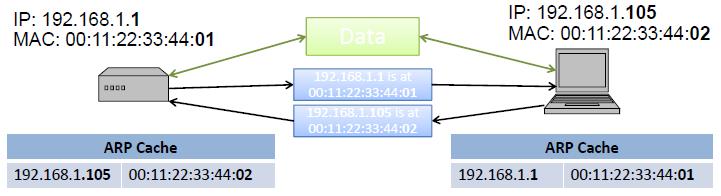
\includegraphics[height=5cm, width=10cm, keepaspectratio]{Immagini/reti/ARP_Caches.png}}
	\caption{ARP Caches\label{fig:ARP_Caches}} 	
\end{figure}
The ARP table is updated whenever an ARP response is received. Notice that requests are not tracked, ARP announcements are not authenticated and machines trust each other, so a rogue machine can spoof other machines.\begin{figure}[htbp]
	\centering%
	\subfigure%
	{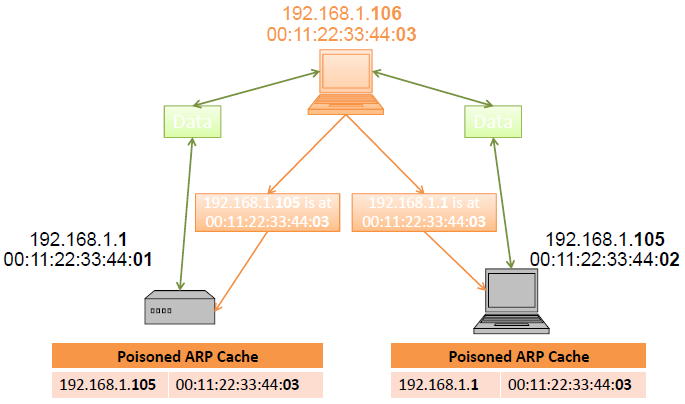
\includegraphics[height=7cm, width=10cm, keepaspectratio]{Immagini/reti/Poisoned_ARP_Caches.png}}
	\caption{Poisoned ARP Caches\label{fig:Poisoned_ARP_Caches}} 	
\end{figure}
According to the standard, almost all ARP implementations are stateless, so an ARP cache (\figurename~\ref{fig:ARP_Caches}) updates every time that it receives an arp reply… even if it did not send any arp request! It is possible to "poison" an ARP cache by sending gratuitous ARP replies (\figurename~\ref{fig:Poisoned_ARP_Caches}). Notice that using static entries solves the problem but it is almost impossible to manage!

\section{Denial of Service Attack}
The DoS Attack (\figurename~\ref{fig:DoS_Attack}) consists in sending large number of packets to an host providing service. This attack, often executed by botnet, slows down or crashes the host. 
\begin{figure}[htbp]
	\centering%
	\subfigure%
	{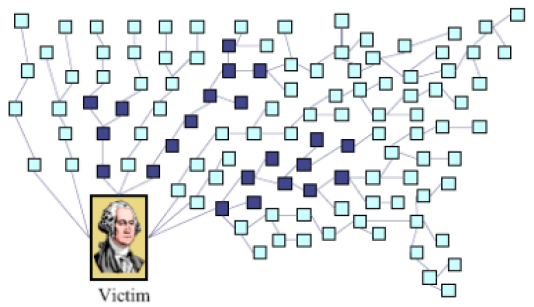
\includegraphics[height=4cm, width=12cm, keepaspectratio]{Immagini/reti/DoS_Attack.png}}
	\caption{DoS Attack\label{fig:DoS_Attack}} 	
\end{figure}
The attack starts at zombies, travels through tree of Internet routers and ends at victim (tree root). The \textbf{IP source spoofing} hides attacker and scatters return traffic from victim.\\ \\
An important problem is to identify leaves of DoS propagation tree (i.e. routers next to attacker). Notice that there are more than 2M Internet routers, attacker can spoof source address and knows that traceback is being performed.\\
Some approaches to this problem could be:
\begin{itemize}
\item Filtering and tracing (immediate reaction)
\item Messaging (additional traffic)
\item Logging (additional storage)
\item Probabilistic marking
\end{itemize}
In particular, probabilistic marking performs random injection of information into packet header, changes seldom used bits, forwards routing information to victim and uses redundancy to survive packet losses. This approach has benefits as:
\begin{itemize}
\item No additional traffic
\item No router storage
\item No packet size increase
\item Can be performed online or offline
\end{itemize}

\subsection{SYN Flood}
SYN Flood is typically a DOS attack, though can be combined with other attack such as TCP hijacking.\\
Rely on sending TCP connection requests faster than the server can process them. Attacker creates a large number of packets with spoofed source addresses and setting the SYN flag on them. The server responds with a SYN/ACK for which it never gets a response (waits for about 3 minutes each); eventually the server stops accepting connection requests, thus triggering a denial of service.
The problem of avoiding this attack can be solved in multiple ways: one of the common way is to use SYN cookies.

\subsection{Optimistic ACK attack}
An optimistic ACK attack takes advantage of the TCP congestion control. It begins with a client sending out ACKs for data segments it hasn't yet received. This flood of optimistic ACKs makes the servers TCP stack believe that there is a large amount of bandwidth available and thus increase congestion window. This leads to the attacker providing more optimistic ACKs and eventually bandwidth use beyond what the server has available. This can also be played out across multiple servers, with enough congestion that a certain section of the network is no longer reachable. Actually, there are no practical solutions to this problem.
